\begin{answer}

\begin{figure}[here]
   \centering
   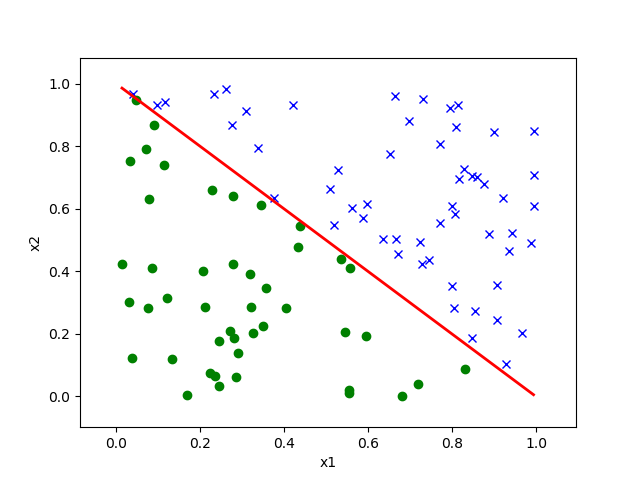
\includegraphics[width=4in]{fig_b.png} 
   \caption{Dataset B}
   \label{fig:separation}
\end{figure}

This figure plots Dataset B. We can see that the two classes [1,0] are well separated.
Separation occurs when variables are associated with only one outcome.
The problem is that when there is separation (the logistic curve lies strictly 0 or 1).
The optimization does not converge,  the model parameter goes to infinity when maximizing the likelihood of the function. The parameters continue increasing, as it tries to find an optimal separation of the classes. However, there is an infinite optimal values in which a linear boundary can form under well separated classes. 

\begin{figure} 
   \centering
   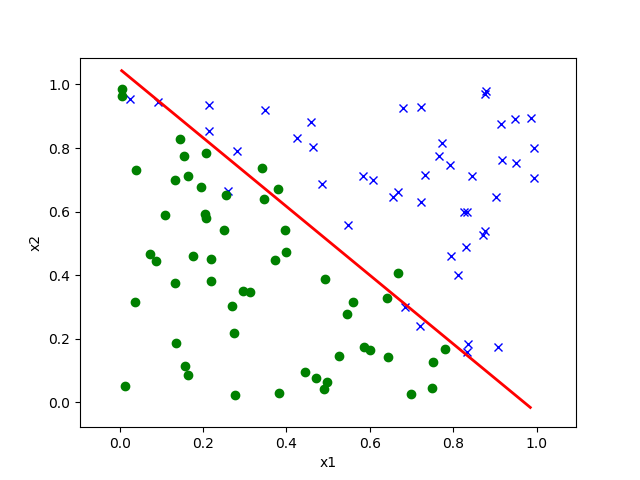
\includegraphics[width=4in]{fig_a.png} 
   \caption{Dataset A}
   \label{fig:separation}
\end{figure}

The Dataset A does not show complete separation of classes.

\end{figure}
